%%%% Paramétrage du TD %%%%
\def\xxactivite{Colle 03 \ifprof -- Corrigé \else \fi} % \normalsize \vspace{-.4cm}
\def\xxauteur{\textsl{Xavier Pessoles}}

\def\xxtitreexo{Régulateur}
\def\xxsourceexo{\hspace{.2cm} \footnotesize{}}
\def\xxauteur{\textsl{Xavier Pessoles}}


\def\xxcompetences{%
\vspace{.25cm}
\textsl{%
\textbf{Savoirs et compétences :}
\begin{itemize}[label=\ding{112},font=\color{ocre}] 
\item \textit{C2-08} :Déterminer les actions mécaniques en dynamique dans le cas où le mouvement est imposé.
\end{itemize}
}}
\def\xxfigures{
%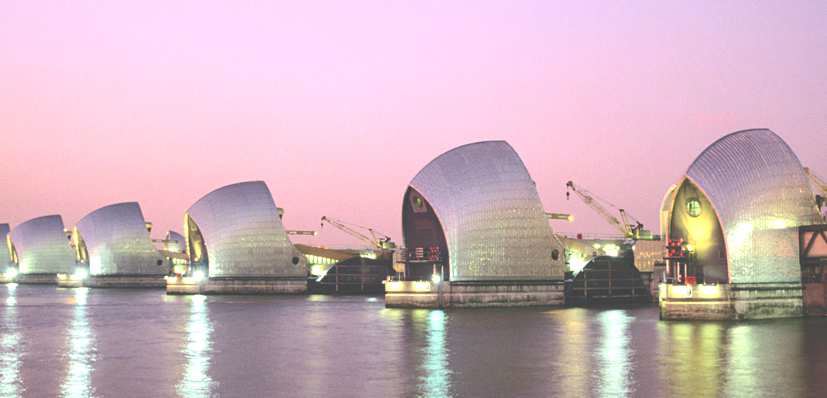
\includegraphics[width=.7\linewidth]{fig_00}
}%figues de la page de garde


\input{\repRel/Style/pagegarde_TD}
\setcounter{numques}{0}

\setlength{\columnseprule}{.1pt}

\pagestyle{fancy}
\thispagestyle{plain}

\vspace{5.1cm}

\def\columnseprulecolor{\color{ocre}}
\setlength{\columnseprule}{0.4pt} 

%%%%%%%%%%%%%%%%%%%%%%%

\setcounter{exo}{0}


\ifprof
\else
\begin{multicols}{2}
\fi


Un système matériel est constitué de 5 solides reliés au bâti \textbf{(0)}. Les solides \textbf{(1)}, \textbf{(2)}, \textbf{(3)} et \textbf{(5)} sont des barres sans épaisseur, articulées par des pivots en $O$, $A$ ou $B$ de manière à demeurer dans un même plan noté $ \left(\vect{x_1},\vect{y_1}\right)$. Cet ensemble est donc mobile en rotation autour de $\vect{z_1}$. On repère sa position angulaire par le paramètre $\psi$. 

Au bâti \textbf{(0)}, on associé le repère fixe $\mathcal{R}_0$. 

À chaque $S_i$ on associe une base $\mathcal{B}_i\base{x_i}{y_i}{z_i}$. Les repère $\mathcal{R}_i$ sont d'origine $O$ ou $A$ selon le cas. 

Les rotations internes sont définies par $\theta_2$ autour de $\axe{O}{y_1}$ et $\theta_3$ autour de $\axe{A}{y_1}$.

Les barres \textbf{(2)} et \textbf{(3)} sont identiques, de longueur $2a$ et de masse $m_2=m_3=m$.

Les barres \textbf{(1)} et \textbf{(5)} ont une masse $m_i$ et des longueurs $\ell_i$. \textbf{(4)} est un volant d'inertie de masse $M$ qui fait l'objet d'une liaison pivot d'axe $\axe{G}{x_3}$ avec la barre \textbf{(3)}. Un repère $\mathcal{R}_4$ est lié à ce volant dont on définit sa position par le paramètre angulaire $\varphi$.

On donne le paramétrage suivant. 

\begin{center}
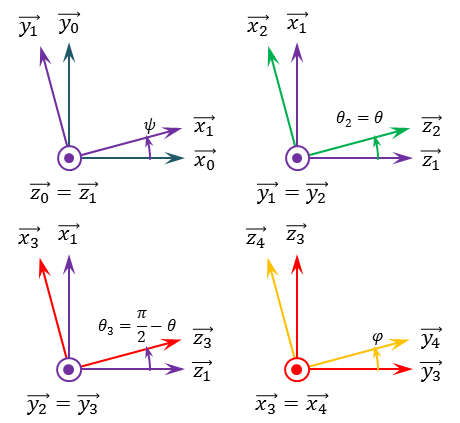
\includegraphics[width=\linewidth]{param2.png}
\end{center}
%
%
%\subparagraph{}
%\textit{Définir le paramétrage cinématique du problème.}
%\ifprof
%\begin{corrige}
%\end{corrige}
%\else
%\fi


\question{Proposer une matrice d'inertie pour chacun des solides.}

\question{Déterminer les torseurs cinétiques suivants : $\torseurci{1}{0}_O$, $\torseurci{2}{0}_O$.}


\question{Déterminer les torseurs dynamiques suivants : $\torseurdyn{1}{0}_O$, $\torseurdyn{2}{0}_O$. En déduire $\torseurdyn{1\cup 2}{0}_O$}


% et  $\torseurci{3}{0}_O$ dans $\mathcal{R}_1$, $\torseurci{4}{0}_O$ dans $\mathcal{R}_3$  et  $\torseurci{5}{0}_A$ dans $\mathcal{R}_1$.}
%=======
%\textit{Proposer une matrice d'inertie pour chacun des solides.}

%\subparagraph{}
%\textit{Déterminer les torseurs cinétiques suivants : $\torseurci{1}{0}_O$, $\torseurci{2}{0}_O$ et  $\torseurci{3}{0}_O$, $\torseurci{4}{0}_O$  et  $\torseurci{5}{0}_A$.}
%>>>>>>> 4ae35b27eb276b13c5159865a72c2d5c28eeea38
\ifprof
\begin{corrige} ~\\

\begin{multicols}{2}
\subsection*{Détermination de  $\torseurci{1}{0}_O$}

$O$ est un point fixe. On a donc :
$$
\torseurci{1}{0}=
\torseurl{
m_1 \vectv{G_1}{1}{0}
}{
\vectmc{O_1}{1}{0} = \inertie{O}{1} \vecto{1}{0}
}{O}
$$

\textbf{(1)} est une tige d'axe $\vect{z_0}$ et de rayon négligeable. On a donc 
$\inertie{O}{1} =  \matinertie{A_1}{A_1}{0}{0}{0}{0}{\mathcal{R}_1} $ avec $A_1=\dfrac{m_1l_1^2}{3}$. 
De plus,
$
\torseurcin{V}{1}{0}=
\torseurl{
\vecto{1}{0}=\dot{\psi}\vect{z_1}
}{
\vectv{O}{1}{0}=\vect{0}
}{O}
$. 
On a donc  $\inertie{O}{1} \vecto{1}{0} =   \matinertie{A_1}{A_1}{0}{0}{0}{0}{\mathcal{R}_1} \begin{pmatrix} 0 \\ 0 \\  \dot{\psi} \end{pmatrix}_{\mathcal{R}_1}=\vect{0}$.
Au final :
$$
\torseurci{1}{0}=
\torseurl{
\vect{0}
}{
\vect{0}
}{O}
$$

\end{multicols}

\begin{multicols}{2}
\subsection*{Détermination de  $\torseurci{2}{0}_O$}

$O$ est un point fixe. On a donc :
$$
\torseurci{2}{0}=
\torseurl{
m_2 \vectv{G_2}{2}{0}
}{
\vectmc{O}{2}{0} %= \inertie{G_2}{1} \vecto{2}{0}
}{O}
$$

\textbf{(2)} est une tige d'axe $\vect{z_2}$ et de rayon négligeable. On a donc 
$\inertie{O_2}{2} =  \matinertie{A_2}{A_2}{0}{0}{0}{0}{\mathcal{R}_2} $ avec $A_2=\dfrac{4ma^2}{3}=$. 
De plus,
$
\torseurcin{V}{2}{0}=
\torseurl{
\vecto{2}{0}=\dot{\psi}\vect{z_1}+\dot{\theta}\vect{y_2}
}{
\vectv{G_2}{2}{0}
}{G_2}
$. 

$\vectv{G_2}{2}{0}=\vectv{O}{2}{0}+\vect{G_2O}\wedge\vecto{2}{0}
=-a\vect{z_2}\wedge \left(\dot{\psi}\vect{z_1}+\dot{\theta}\vect{y_2}\right)
=a \left(\dot{\psi}\sin\theta\vect{y_1}+\dot{\theta}\vect{x_2}\right)
=a \left(\dot{\psi}\sin\theta\vect{y_1}+\dot{\theta}\left( \cos\theta \vect{x_1}-\sin\theta \vect{z_1}\right)\right)$

On a donc 

$\inertie{O_2}{2} \vecto{2}{0} =   \matinertie{A_2}{A_2}{0}{0}{0}{0}{\mathcal{R}_2} \begin{pmatrix} -\dot{\psi}\sin\theta \\ \dot{\theta} \\  \dot{\psi}\cos\theta \end{pmatrix}_{\mathcal{R}_2}=
 \begin{pmatrix} -A_2\dot{\psi}\sin\theta \\ A_2\dot{\theta} \\  0 \end{pmatrix}_{\mathcal{R}_2}$.
 
 
Au final :
$$
\torseurci{2}{0}=
\torseurl{
ma\begin{pmatrix}
 \dot{\theta}\cos\theta\\
 \dot{\psi}\sin\theta \\
 -\dot{\theta}\sin\theta
\end{pmatrix}_{\mathcal{R}_1}
}{
\begin{pmatrix} -A_2\dot{\psi}\sin\theta \\ A_2\dot{\theta} \\  0 \end{pmatrix}_{\mathcal{R}_2}
}{O}
%$$
%$$
%\torseurci{2}{0}=
%\torseurl{
%ma\begin{pmatrix}
% \dot{\theta}\cos\theta\\
% \dot{\psi}\sin\theta \\
% -\dot{\theta}\sin\theta
%\end{pmatrix}_{\mathcal{R}_1}
%}{
%\begin{pmatrix} -A_2\dot{\psi}\sin\theta \\ A_2\dot{\theta} \\  0 \end{pmatrix}_{\mathcal{R}_2}
%}{O}
%$$
%
%$$
%\torseurci{2}{0}
=
\torseurl{
ma\begin{pmatrix}
 \dot{\theta}\cos\theta\\
 \dot{\psi}\sin\theta \\
 -\dot{\theta}\sin\theta
\end{pmatrix}_{\mathcal{R}_1}
}{
\begin{pmatrix} 
-A_2\dot{\psi}\sin\theta\cos\theta \\ 
A_2\dot{\theta} \\  
A_2\dot{\psi}\sin\theta\sin\theta 
\end{pmatrix}_{\mathcal{R}_1}
}{O}
$$

\end{multicols}



\begin{multicols}{2}
\subsection*{Détermination de  $\torseurci{3}{0}_O$}
******************
Au point $G_3$, on a :
$$
\torseurci{3}{0}=
\torseurl{
m_3 \vectv{G_3}{3}{0}
}{
\vectmc{G_3}{3}{0} %= \inertie{G_2}{1} \vecto{2}{0}
}{O}
$$

\textbf{(3)} est une tige d'axe $\vect{x_3}$ et de rayon négligeable. On a donc 
$\inertie{G_3}{3} =  \matinertie{0}{B_3}{B_3}{0}{0}{0}{\mathcal{R}_3} $ avec $A_4=\dfrac{4ma^2}{3}=$. 
De plus,
$
\torseurcin{V}{3}{0}=
\torseurl{
\vecto{3}{0}=\dot{\psi}\vect{z_1}+\dot{\theta}_3\vect{y_3}
}{
\vectv{G_3}{3}{0}
}{G_3}
$. 

$\vectv{G_3}{3}{0}
%=\vectv{O}{2}{0}+\vect{G_2O}\wedge\vecto{2}{0}
%=-a\vect{z_2}\wedge \left(\dot{\psi}\vect{z_1}+\dot{\theta}\vect{y_2}\right)
%=a \left(\dot{\psi}\sin\theta\vect{y_1}+\dot{\theta}\vect{x_2}\right)
%=a \left(\dot{\psi}\sin\theta\vect{y_1}+\dot{\theta}\left( \cos\theta \vect{x_1}-\sin\theta \vect{z_1}\right)\right)$
$

On a donc 

$\inertie{O_2}{2} \vecto{2}{0} =   \matinertie{A_2}{A_2}{0}{0}{0}{0}{\mathcal{R}_2} \begin{pmatrix} -\dot{\psi}\sin\theta \\ \dot{\theta} \\  \dot{\psi}\cos\theta \end{pmatrix}_{\mathcal{R}_2}=
 \begin{pmatrix} -A_2\dot{\psi}\sin\theta \\ A_2\dot{\theta} \\  0 \end{pmatrix}_{\mathcal{R}_2}$.
 
 
Au final :
$$
\torseurci{2}{0}=
\torseurl{
ma\begin{pmatrix}
 \dot{\theta}\cos\theta\\
 \dot{\psi}\sin\theta \\
 -\dot{\theta}\sin\theta
\end{pmatrix}_{\mathcal{R}_1}
}{
\begin{pmatrix} -A_2\dot{\psi}\sin\theta \\ A_2\dot{\theta} \\  0 \end{pmatrix}_{\mathcal{R}_2}
}{O}
=
\torseurl{
ma\begin{pmatrix}
 \dot{\theta}\cos\theta\\
 \dot{\psi}\sin\theta \\
 -\dot{\theta}\sin\theta
\end{pmatrix}_{\mathcal{R}_1}
}{
\begin{pmatrix} 
-A_2\dot{\psi}\sin\theta\cos\theta \\ 
A_2\dot{\theta} \\  
A_2\dot{\psi}\sin\theta\sin\theta 
\end{pmatrix}_{\mathcal{R}_1}
}{O}
$$

\end{multicols}


\end{corrige}
\else
\fi

\question{Déterminer les torseur dynamique $\torseurdyn{4}{0}_G$.}
\ifprof
\begin{corrige}
\end{corrige}
\else
\fi

\question{Déterminer les torseur dynamique $\torseurdyn{1\cup 2\cup 3\cup 4\cup 5}{0}_O$.}
\ifprof
\begin{corrige}
\end{corrige}
\else
\fi


\question{Calculer l'énergie cinétique de l'ensemble du système dans son mouvement par rapport au bâti.}
\ifprof
\begin{corrige}
\end{corrige}
\else
\fi



\begin{center}
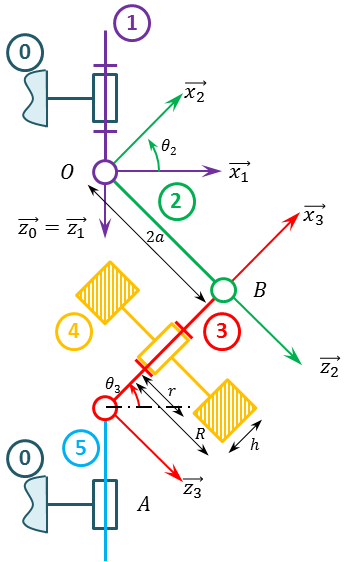
\includegraphics[width=\linewidth]{Schema_Cin.png}
\end{center}


\ifprof
\else
\end{multicols}
\fi



